\section{}
Consider a cylinder rolling on a board, with a torque applied to the latter:
\begin{figure}[h]
    \centering
    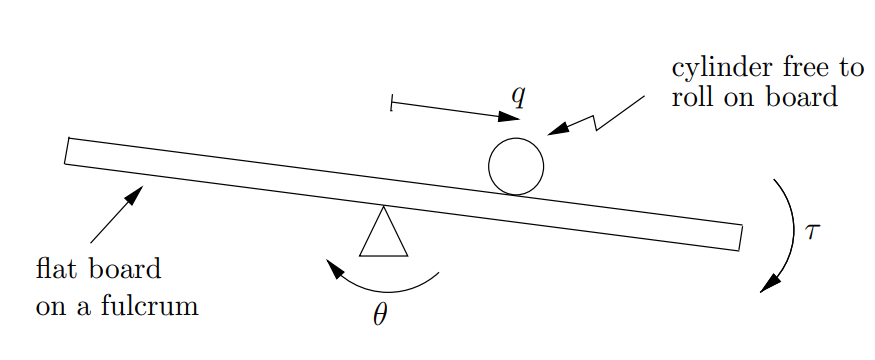
\includegraphics[width=0.5\textwidth]{Questions/Figures/Q4ProblemDiagram.png}
    \caption{Cylinder rolling on a board.}
    \label{fig:Q4 System}
\end{figure}

% As shown, the angle of tilt is denoted by θ, the torque applied to the board is τ , and q measures the
% distance the cylinder rolls down the board. Let J denote the mass moment of inertia of the board
% about its pivot and Jc, Rc and Mc the mass moment of inertia, radius and mass of the cylinder,
% respectively. Assuming roll without slip, the equations of motion can be shown to be
% write in mathmode

As shown, the angle of tilt is denoted by $\theta$, the torque applied to the board is $\tau$, and $q$ 
measures the distance the cylinder rolls down the board. Let $J$ denote the mass moment of inertia of the board 
about its pivot and $J_c$, $R_c$ and $M_c$ the mass moment of inertia, radius and mass of the cylinder, 
respectively. Assuming roll without slip, the equations of motion can be shown to be:

\begin{align}
    &\left(\frac{J_c}{R_{c}^2} + M_c\right)\ddot{q} + M_{c}g \sin{\theta} - M_{c}q \dot{\theta}^2 = 0 \label{eq: Q4a1} \\
    &(M_{c}q^2 + J + J_c)\ddot{\theta} + 2M_{c}q \dot{q} \dot{\theta} + M_{c}gq \cos{\theta} = \tau \label{eq: Q4a2}
\end{align}

\subsection{}
\textit{What is the order of this system?}

The system consists of two 2nd order differential equations, so the order of the system is 2.
\subsection{}
\textit{Defining $x = (q, \theta, \dot{q}, \dot{\theta})$, $u = \tau$ and $y = q$, write the state model of this system.}

Isolating the $\ddot{q}$ and $\ddot{\theta}$ terms in (\ref{eq: Q4a1}) and (\ref{eq: Q4a2}) respectively, we get:

\begin{align*}
    \ddot{q} &= \frac{1}{\frac{J_c}{R_{c}^2} + M_c} \left(M_{c}q \dot{\theta}^2 - M_{c}g \sin{\theta}\right) \\
    \ddot{\theta} &= \frac{1}{M_{c}q^2 + J + J_c} \left(u - 2M_{c}q \dot{q} \dot{\theta} - M_{c}gq \cos{\theta}\right)
\end{align*}

The state model is therefore:
\begin{empheq}[box=\fbox]{align*}
    \dot{x} &=
    \begin{bmatrix}
        \dot{q} \\
        \dot{\theta} \\
        \frac{1}{\frac{J_c}{R_{c}^2} + M_c} \left(M_{c}q \dot{\theta}^2 - M_{c}g \sin{\theta}\right) \\
        \frac{1}{M_{c}q^2 + J + J_c} \left(u - 2M_{c}q \dot{q} \dot{\theta} - M_{c}gq \cos{\theta}\right)
    \end{bmatrix} \\
    y &= q
\end{empheq}

\subsection{}
\textit{Does the system in (b) have a state-space form? Why or why not?}

The system in (b) does not have a state-space form because the state dynamics are not linear due to the presence of 
the $q^2$, $\sin{\theta}$, $\cos{\theta}$, $\theta^2$, $2M_{c}q \dot{q} \dot{\theta}$, and various other non-linear terms.
    
        

